\documentclass [11pt, a4paper]{report}
\pagestyle{headings}
\usepackage{nomencl}
\usepackage{graphicx}
\usepackage{url}
\usepackage[pdftex]{hyperref}
\begin{document}

\pagestyle{empty}
%\noindent 

\begin{figure}[hp]
\centering
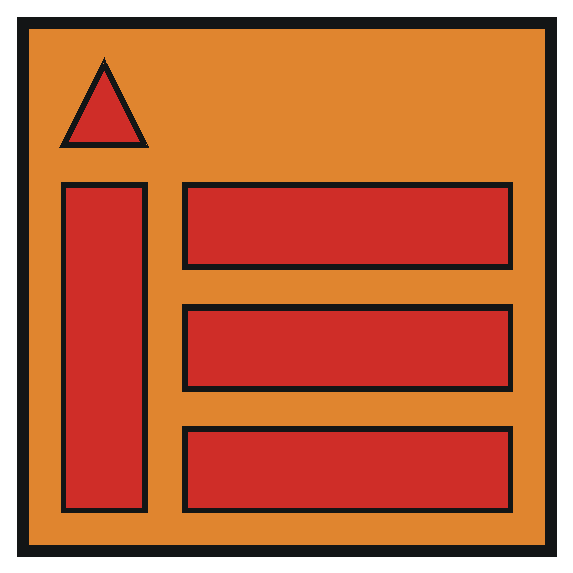
\includegraphics[height=20mm, clip]{figures/inso-farbe}
\hspace{1mm}

\includegraphics[height=20mm, clip]{figures/info-farbe}
\hspace{1mm}

\includegraphics[height=20mm, clip]{figures/tu-dt-teil-schw-pos}
\label{fig:TU-Wien}
\end{figure} 

\bigskip
\bigskip

\begin{center}
    \huge\bfseries
  Thermal Tumor Ablation
\end{center}

\bigskip
\bigskip

\begin{center}
  \Large
  \centering Bachelor of Science Thesis
\end{center}

\medskip

\begin{center}
  submitted for the academic degree of \\
  Bachelor of Science (B.Sc.)
\end{center}

\medskip

\begin{center}
  carried out at the\\
  Research Group for Industrial Software\\
  Institute of Computer Aided Automation\\
  Vienna University of Technology
\end{center}

\begin{center}
  under the guidance of\\
  Mag. DI Dr. Wolfgang Schramm
\end{center}

\begin{center}
  by\\
  Haichao Miao \\
  Hirtenberger Stra�e 24b \\
  2544 Leobersdorf \\
  hmiao87@gmail.com
\end{center}

\bigskip
\bigskip
\bigskip
\bigskip

\begin{center}
  Vienna, \today
\end{center}

\vspace*{\fill}

\cleardoublepage

\rmfamily
\normalfont

\noindent
\emph{Optional: Put your favorite quote here}
\begin{flushright}
Optional: Author of quote
\end{flushright}
% *************** Table of contents ***************
\pagenumbering{roman}
\pagestyle{headings}
\tableofcontents

% *************** End of front matter ***************

\pagestyle{headings}

\pagenumbering{arabic}

\chapter*{Abstract}
Thermal ablation as a treatment for tumors has been established continuously over the past years. It offers a complementary treatment to eliminate or shrink tumors in a minimal invasive way with significant lower risk of major complications. Medical imaging device has become indispensable for accomplishing thermal ablation. The first chapter of this thesis gives an overview of image-guided ablation techniques including radiofrequency (RFA), cryotherapy and microwave. \\

Since thermal ablation is a complex procedure and because of the collaboration of several specialists during the intervention, there is a need for a planning platform which supports the specialists in planning the ablation. Thereby the second chapter discusses the implementation of a thermal ablation software prototype which allows the collaborators to simulate and plan the ablation (RFA and cryotherapy) before the actual intervention on basis of the patient's specific anatomy. 

\chapter*{Zusammenfassung}
Hier die deutsche Zusammenfassung einf�gen

\chapter*{Acknowledgements}
Your acknowledgements to...

% include chapters here

\chapter*{Introduction}

%patient selection, indicators etc. see dodd.pdf
% see dodd.pdf for additional infos

\chapter{Image-guided Thermal Ablation Techniques}
\section{Introduction}

\subsection{Overview}
Different ablation methods are used in clinical environment. The decision which method is going to be used, not only depends on the tumor location, but also on the geographical region where it comes to use This chapter compares the different thermal ablative techniques in tumor therapy that are commonly used. 
\\
Although the rapid advancement in ablative techniques has taken place within the past 20 years, experiments with ablation of tissues using radiofrequency (RF) has been already documented at the end of the 19th century \cite{filingery2005}. 

What all ablative techniques in general have in common is, they attempt to kill every viable malignant cell within the designated area using thermal energy sources in a minimally invasive manner. At the same time minimal damage to the surrounding organs is done. There are several ways to accomplish this, but they can generally divided into two groups, based on whether heating or freezing is utilized to kill tumor cells \cite{ahmed-basic}. Currently the most common method is Radiofrequency Ablation, but other techniques are coming more and more to use. Cryoablation is used effectively in the treatment of prostate and kidney cancer. Microwave Ablation (MWA) is widely used in the Asian region. Especially Microwave Ablation has shown high potential in treating pulmonary tumors due to the significant larger ablation zone compared with RF \cite{brace-microwave}. 

Other thermal energy sources are Laser and High-intensity Focused Ultrasound. 
\\
Chemical substances can also be used to kill tumor cells. Chemical Ablation was documented being efficient in destroying hepatocellular carcinoma (HCC). Thereby chemical ablative substances (e.g. ethanol or acetic acid) are injected into the tumor  \cite{ahmed-basic}. These techniques will not be in the main focus of this thesis.

\subsection{Image Guidance and Minimal Invasiveness}

The ablation of tumor with thermal energy sources (in literature also referred as tumor ablation) represents the non-surgical alternative solution for patients with cancer. Especially with the rapidly increasing advancement in imaging technologies, the techniques became lesser invasive. Even during an intraoperative procedure imaging techniques, such as intraoperative ultrasound, are necessary. Hence imaging is essential during the ablation process, since the interventional radiologist utilizes it to target the tumor inside the patients body. Depending on the imaging modality and tumor properties, surgery is often not required. 

\begin{figure}[htb]
\centering
\includegraphics[width = 80mm]{images/liver-us.jpg}
\caption{Tumor ablation intervention under Ultrasound-guidance with CT scans of the patient before and after the ablation. Image taken from \cite{dodd-2000}}
\label{fig:liver-us}
\end{figure}

% Image monitoring
% Postinterventional...

% (also in planning and post.. controlling)

% need better phrasing
\subsection{Benefits of Thermal Ablation}
The increasing application of thermal ablation demonstrates the benefits from thermal ablation. 
\begin{itemize}
\item Minimal invasiveness. Small probes are punctuated through the skin into the center of the tumor (percutanous). Due to imaging technologies, there is no need to cut through the skin in most cases. 
\item Compared to surgery, there are less complications reported during and after the procedure. % citation needed
\item Re-treatment possible. This is especially relevant when metastases reappear. 
\item Less tissue is removed compared to surgical resection, because only the tumor and a safety margin of 1cm have to be ablated.
\item Alternative to surgery. Patients who are not surgical candidates or patients with few small Tumors are qualified for thermal ablation. 
\end{itemize}


% ... not alone by doctor. radiologist + assistance of technologies

% procedure

\section{Overview: Thermal Ablation Techniques}

Thermal ablative techniques differ mainly by their method of generating heat or cold. 
%need more here

\subsection{Radiofrequency Ablation}

% zitat bitte auf original �ndern
Since the early 1990 there has been enormous development of percutaneous Radiofrequency technology \cite{helmberger-rfa}. RFA as a treatment for primary and secondary hepatic malignancies has been performed successfully for more than 10 years. But there has also been reports for RFA treatment for nearly all kinds of tumors. 

\subsubsection{Technique of Radiofrequency Ablation}

In RFA high-frequency alternating current (typically between 450 - 500 kHz) is applied through an electrode into the biological tissue. Thereby an electric field within the tissue is established which oscillates with the applied radio frequency inducing ionic friction. When enough energy is deployed over a certain amount of time, the ionic friction results in loss of heat energy, which emerges into the tissue by the phenomena of convection. A coagulative necrosis follows. 

% figure shows the interdependency of temperature and radius. 
% charring

The efficacy of the RFA and the resulting size of the coagulation zone depends on the following factors \cite{helmberger-rfa}: 

\begin{itemize}
\item amount of energy deployed
\item duration of exposure
\item electrode design
\item tissue-specific factors (heat connectivity and conversion)
\item "heat sink" and "oven effect" %explain?
\end{itemize}

\subsubsection{Electrodes}

As mentioned before, the RF current is deployed through an electrode directly into the tissue. In general these electrodes consists of an isolated shaft and an active tip. Various electrodes creates different coagulation volume shapes, mostly between 2 and 5 cm in diameter. 

\subsubsection{Radiofrequency Generators}

The ablation process is controlled over the generator. Concerning the above mentioned tissue-specific and other factors, the amount and duration of energy exposure has to be well adapted for the tumor. The process is thereby very device-dependent. Thus the personal experience of the operator is essential to ensure efficient treatment of the disease \cite{poon-rf}.

% Figure

\subsubsection{Procedure}

RFA is usually performed under conscious sedation. Ultrasound (US), computed tomography (CT) and magnetic resonance imaging (MRI) are normally used for targeting the probe into the tumor and monitoring the result. It usually takes more than one placement, especially when several tumors has to be targeted. 


These imaging methods has both advantages and disadvantages. US is the most used worldwide, because with this setting no radiologist is required for the procedure. 
CT is the most used imaging modality by interventional radiologist \cite{helmberger-rfa}. It has anatomically exact imaging and is widely available. Though MRI guidance has high contrast tumor-to-tissue, it has the necessity for MR-compatible equipment \cite{diss-schramm}. This circumstance does not exclude MRI, but it is often the reason for using other imaging modalities. 

RFA is perceived by some clinicians as a simple treatment form, where simply just by inserting a needle and "cooking" the tumor \cite{poon-rf}. As showed above, the procedure is more complex and the efficacy of the treatment is dependent on many factors. 

\begin{figure}[htb]
\centering
\includegraphics[width = 130mm]{images/rfa-strategies.jpg}
\caption{The figures show the spherical thermal injuries done by the different RFA treatment strategies. Tumors less than 2cm can be treated with a single ablation, larger tumors in size need to be performed multiple times \cite{dodd-2000}. Images taken from \cite{dodd-2000}}
\label{fig:rfa-strategies}
\end{figure}

%complications (maybe a summary for all techniques) 
%majo clinic

\subsubsection{Conculusion}

Studies has shown Radiofrequency Ablation to be an effective, safe and low-risk technique for treating liver tumors. It has come more and more to use over the past years. 

RFA is a technology-based treatment form and efficient application is thereby highly dependent on the experience of the operator. Due to the treatment's interdependence on various factors and its highly conjunction with technology, it can be assumed that a planning phase is necessary. 

\subsection{Cryoablation}

The destruction of tissue by freezing is one of the oldest methods of tissue destruction known to mankind \cite{mortele-mri}. But substantial progress in destroying cancer tissue has been made not until recently. 
In the 60s, nitrogen-cooled probes for cryotherapy established in hepatic surgery. Probes were relatively large in size and open surgical was necessary for the placement of the probe \cite{silverman-cryo}. The development of smaller percutaneous cryoprobes, using argon gas eliminated the risks associated with open surgery \cite{ahmed-basic}.
Currently Cryoablation (CA) is been successfully used to treat several types of tumor. 

The major advantage of CA is the clear visualization of the iceball generation under different imaging modalities. This ensures precise monitoring and therefore better control of the ablation zone dimension. 

\subsubsection{Technique of Cryoablation}

In order to treat effectively and have control over the process the operator has to understand the mechanisms of cryogenic injury. In recent years freezing has not only used to destroy tissue, but also to preserve. The cell destruction with freezing is achieved by two major mechanisms. Cells are injured by ice crystal formation and the microcirculary failure, which occurs in the thawing period \cite{gage-cryo}. At low freezing rates, the freezing propagates through the extra-cellular space, which causes water to be drawn from the cell and cell results in osmotic dehydration \cite{ahmed-basic}. 
At faster freezing rates, intra-cellular ice crystal formation causes lethal damages to organelles and membrane \cite{ahmed-basic}.

\subsubsection{Devices}

As mentioned before, the development of argon-based systems replaced liquid nitrogen units, because argon has major advantages to nitrogen. As an example, Argon-based systems circulate very fast and as a result, iceball formation emerge very quickly. Probe tips of these systems reach temperatures around -150 �C. 

The two Cryoablation systems available in the United States are CRYOcare (EndoCare inc., Irvine, California) and CryoHit (Galil Medical Ltd., Wallingford, CT) \cite{sharon-cryo}. The latter is the only unit with MRI compatible cryoprobes \cite{cryohit}. They are both argon-based and use simultaneously multiple probes for the placement in the shape of the tumor in order to cover it. 

\subsubsection{Probes}

Both of above mentioned systems use eight sharp-tipped cryoprobes, that can directly place into the tumor. CRYOcare uses 2.4-4.9mm OD probes and CryoHit 1.4-3.4mm probes. 

\begin{figure}[htb]
\centering
\includegraphics[width = 80mm]{images/cryo-tips.jpg}
\caption{The picture shows the ellipsoidal ice ball formation around the probe tip (Galil Medical, Yorkneam, Israel). Picture taken from \cite{silverman-cryo}.}
\label{fig:cryo-tips}
\end{figure}

\subsection{Microwave Ablation}

Microwave Ablation (MWA), the latest development in tumor ablation, has been shown to have potential advantages over RFA, which is the most extensively applied modality. Zones of ablation are significantly larger and therefore faster treatment time can be achieved, compared to RFA. Yet, there is no approved device for patient treatment within the USA or Europe but in the Asian region devices has been developed since the early 90s  \cite{boss-mwa}.

\subsubsection{Technique of Microwave Ablation}

In Microwave Ablation tissue heating and resulting cell death is induced by high-frequency electromagnetic waves in the GHz order. Microwaves has wavelengths between infrared light and radio waves. 
Similar to RFA, a microwave antenna is placed into the tumor and emits electromagnetic microwaves into the surrounding tissue. It causes water molecules with an electric dipole moment to align themselves to the alternating electric field induced by microwaves. These oscillations of water molecules inside the cells results in warming. Macromolecules are not effected by microwaves but they are heated by convection nonetheless resulting in coagulation necrosis.

Although water molecules has a resonance frequency of ca. 22,2 GHz, they typically absorb 50\%-60\% of electromagnetic energy effectively in the range of 1-2 GHz \cite{boss-mwa}. Hence newly developed MWA devices work at frequencies below 1 GHz and use several applicators at the same time. 

\subsubsection{Devices}

As mentioned before, MWA devices for patient treatment has only applied in Asia so far. Figure \ref{fig:microtaze} (left) shows a japanese MW generator with generating power of 150 W. The chinese device (UMC-I Ultrasound-Guided Microwave Coagulator, Institue 207 Aerospace Industry Company, Beijing, China, and Department of Ultrasound of Chinese PLA General Hospital, Beijing, China) with generating power up to 80 W \cite{lu-mwa, boss-mwa}. Both operates at 2.450 MHz emission frequency. 


\begin{figure}[htb]
\centering
\includegraphics[width = 80mm]{images/microtaze.png}
\caption{Microtaze (Heiwa, Osaka, Japan) and needle electrodes. Taken from  \cite{dodd-2000}}
\label{fig:microtaze}
\end{figure}

\begin{figure}[htb]
\centering
\includegraphics[width = 80mm]{images/umc.png}
\caption{"Multiple electrode insertion technique. Five guiding needles are inserted, then microwave energy is applied with one needle at a time." Taken from \cite{lu-mwa}}
\label{fig:umc}
\end{figure}

\subsubsection{Electrodes}

The japanese system uses electrodes with 1.6 mm in diameter and a 2-cm active tip, the chinese system 1.6 mm with a 2.7-cm tip. 

\subsection{Laser Ablation}

Laser-induced Thermotherapy (LITT) is another minimal invasive thermal ablative technique. High energy laser radiation is applied through optical fiber directly into the tumor and energy absorption leads to heating and consequently to tissue destruction. 
Since laser light is used instead of RF, MR imaging is compatible with LITT devices. This circumstance assures real-time monitoring of the status of the intervention, due to the good soft-tissue contrast and high spatial resolution of MR imaging. Another advantage is the preservation of a well-defined area of necrosis around the fiber tip and thus minimal damage is done to the surrounding tissue \cite{laser-mack}. 

Although LITT is a suitable technique for local tumor destruction within solid organs, it is mostly used for the destruction of primary and secondary liver tumors. 

\subsubsection{Technique of Laser Ablation}

Laser light with a wavelength between 1060 and 1200nm is transmitted though a MR-compatible probe to the tissue which leads to coagulation necrosis \cite{laser-vogl}. Photons of this wavelength has a deep penetration depth. The penetration depth of photons is not only depended on the wavelength, but also dependent on the tissue. The interaction between biological tissue and laser light is controlled by many physical phenomena, but at these small amount of energy, that is used in LITT, only scattering and absorption has effective influence on the process. Thanks to the effect of thermal conduction, the temperature extends into the tissue. 
The laser light itself is transmitted via optical fiber. The applicator holds magnetite markers to allow easier visualization and positioning during the intervention \cite{laser-mack}.

\subsubsection{Devices}

Most LITT devices use a neodynium: yttrium-aluminum-garnet (Nd:YAG) laser source. Devices differ in design, types and size of optic fibers, probe tip design and the number of applicators. 
The MediLas 5100 (Dornier MedTech) uses Nd:YAG lasers with a wavelength of 1064nm. The laser is delivered through a specially developed flexible diffusing applicator. 

\begin{figure}[htb]
\includegraphics[width = 80mm]{images/medilas5100.jpg}
\caption{Dornier MediLas 5100 laser system. Picture taken from \cite{img-litt2}}
\label{fig:medilas5100}
\end{figure}

\begin{figure}[htb]
\includegraphics[width = 50mm]{images/flexibleapplicator.jpg}
\caption{The MediLas 5100 flexible applicator. Picture taken from \cite{img-litt1}}
\label{fig:flexibleapplicator}
\end{figure}

\subsection{High-intensity Focused Ultrasound}

High-intensity focused ultrasound (HIFU) is currently studied as a potential method for noninvasive destruction of localized tumors. The main advantage of using HIFU is the noninvasiveness of this treatment. With a transducer ultrasound creates a focused energy beam from the distance. 
Ultrasound, as form of vibrational energy propagates through the tissue as a mechanical wave. At the targeted point, the beams interfere in a hot spot and result in coagulation necrosis.  

\begin{figure}[htb]
\includegraphics[width = 70mm]{images/HIFU.png}
\caption{Schematic of HIFU treatment. Ultrasound is bundled in a focal point, where it results in heating. Image taken from \cite{img-hifu}}
\label{fig:hifu}
\end{figure}


\subsection{Shapes of Ablation Zones}

%short introduction

\begin{center}
\begin{tabular}{ | l | l | l | l |}
    \hline
	Probe & Number of Applicators & Shape & Technique \\ \hline
	Cool Tip & single needle\footnotemark[1] & ellipsoid\footnotemark[1] & RFA  \\ 
	Cool Tip Cluster & cluster electrodes\footnotemark[1] & ellipsoid\footnotemark[1] & RFA  \\ 
	LeVeen & multi-tined electrodes\footnotemark[1] & spherical\footnotemark[1] & RFA  \\ 
	Starburst XL & multi-tined electrodes\footnotemark[1] & pear\footnotemark[1] & RFA  \\ 
	Rita & perfused Talon needle\footnotemark[1] & pear\footnotemark[1] & RFA  \\ 
	Celon (Olympus) & single needle\footnotemark[1] & ellipsoid\footnotemark[1] & RFA  \\ 
	Microblate & single electrode & spherical\footnotemark[2]  & MWA   \\ 
	Microtaze & single electrode & ellipsoid\footnotemark[3]  & MWA   \\  % brochure
	IceSeed & single needles & spherical\footnotemark[4]  & CA   \\  % brochure
	IceSphere & single needles & ellipsoid\footnotemark[4] & CA   \\   % brochure
	IceRod & single needles & ellipsoid\footnotemark[4] & CA   \\   % brochure
	IceBulb & single needles & bulb\footnotemark[4] & CA   \\  \hline % brochure
\end{tabular}

\end{center}
\footnotetext[1]{\cite{helmberger-rfa}}
\footnotetext[2]{\cite{mw-jones} }
\footnotetext[3]{\cite{microtaze}}
\footnotetext[4]{\cite{cryohit}}

\subsection{Requirement for a Planning Platform for Thermal Ablation}

Thermal Ablation Techniques are gaining popularity as a complementary choice of therapy for different tumors. Although it is commonly considered a safe and low-risk technique, it still suffers from a noticeable rate of complications. A review showed that complication rate of RFA for liver tumors are higher than previously assumed \cite{mulier-rfa}. RFA treatments still has higher tumor recurrence rate than surgical resection. The procedure is more complex as it appear at first. It is not simply inserting a needle and "cook" the tumor \cite{poon-rf}.
The treatment outcome of an intervention is highly influenced by different factors:
\begin{itemize}
\item The placement of the applicator(s) is by far the most time-consuming part of the process. Tumors larger in size or multiple small tumors require repeated applicator placement and ablation.
However the accurate placement is essential for the efficient treatment. 
\item The imaging modalities for the guidance of the applicator placement and monitoring the developing ablation zone. Ultrasound is the most frequently used modality, but it is inadequate for imaging the ablation zone accurately \cite{diss-schramm} 
\item Larger tumors require lager ablation zones, but this is accompanied by loss of control with an increased rate of damage to healthy tissue. 
\item Tumors adjacent to large vessels are more difficult to ablate completely since the blood flow acts like a heat sink (see heat sink effect).
\item Since thermal ablation techniques are technology-based treatments, the outcome is highly dependent on the wide variation of probe devices, imaging modalities and experience of the operator with these technologies. 
\end{itemize}

The accurate estimation of the ablation zone and treatment result is essential for the success of the intervention. Due to the fact that the above mentioned factors has great influence on the outcome of a thermal ablation intervention, it can be assumed that using a Planning Platform for Thermal Ablation Techniques will positively affect the outcome. This system estimates the ablation zone based on the patient-specific anatomy using 3D visualization and virtually place applicators. \\

% todo: heat sink effect

\subsection{Conclusion}

Thermal ablation techniques have been developed within the last years as technological advances were made. They are used in clinical practice for the treatment of different localized tumors. Shorter hospital stay, lesser complication during the procedure compared to surgical resection are some of the advantages of these techniques.

Radiofrequency Ablation is the most commonly used technique, followed by Cryoablation and Microwave Ablation. Each technique has advantages and disadvantages. However there are still very little textbook knowledge for education and practice available \cite{diss-schramm}. In addition the theoretical work of the simulation of the ablation zone is advanced (e.g. see FEA), but they use generic models instead of taking the patient's anatomic structure into account \cite{diss-schramm}. Due to these circumstances and the strong interconnection between medical practice and technology is most likely that benefits from treatment simulation can be derived. 

% eine enge verbindung zwischen technologie und behandlungsmethoden.
% generell geringe krankenhaus aufenthalt und weniger komplikationen
% malignant cells are more sensitive
% outcome prediction

\chapter{Requirement Analysis for a Patient Specific Planning-Software}

\section{Introduction}

A platform that is targeted to plan the thermal ablation procedure needs to fulfill a minimum set of features. The finished application should help the operator to plan the intervention. But besides the basic functional requirements there is also the non-functional features. As in all software projects, these are as important as functional features. Especially when the software is used in clinical practice, it has to meet usability and formal requirements. All organizational and formal requirements would go beyond the scope of this thesis and therefore will not be examined in detail. 
\\
In software engineering, a functional requirement is described as specific behavior of a software system, that defines what a system is supposed to accomplish \cite{wiki-functional}. In contrast non-functional requirements defines how a system is supposed to be, e.g. qualities of a system \cite{wiki-nonfunctional}.

Dr. Wolfgang Schramm has reviewed the requirements on such a system in his PhD thesis and therefore the planning software is mostly based on the requirement analysis did by him. In his PhD thesis he discussed the problems between accurate forecast of the treatment outcome and usability. Schramm describes the use of Finite Element Analysis (FEA), that simulates the treatment outcome of thermal ablation, but the additional medical benefit is still not studied \cite{diss-schramm}. Furthermore the detailed simulation requires high computing power, which leads to a very time-consuming process. That makes distinct forecast not feasible to perform during or immediately before the intervention \cite{diss-schramm}. 


\section{Functional Requirements}

\subsection{Image Analysis, Image Processing and Visualization}

Thermal ablation is an image-guided therapy and therefore imaging plays a main role in the application. Given that the simulation is based on the patient specific data, the application has to load the  data in order to simulate the intervention adequately. Since \gls{dicom} is an open standard, that is implemented by nearly all manufacturers of medical imaging devices, the application must load at least DICOM volumes. For further using, the DICOM volume has most likely to be post-processed. The physician needs to perform simple image processing algorithms to image registration and segmentation for high quality treatment planning \cite{diss-schramm}. 

The visualization of the structures is essential to view and interpret the outcome of the treatment. Due to this fact, visualization makes a major part of the functionality of the application. Not only the segmented structures, but also the 3D model of the applicator and the virtual resulting ablation zone have to be visualized. 

\subsection{Treatment Simulation}

The main function of the tool is to provide an adequate forecast of the treatment outcome. Since the resulting ablation zone is highly dependend on the used devices, it is necessary to use 3D models of the real devices for the simulation. Thus one of the main requirements is to make sure that the operator can use the 3D model devices with the same properties as the real ones. 

The actual ablation outcome is very hard to forecast due to the perfusion mediated temperature change during the ablation \cite{diss-schramm}. As mentioned in the introduction of this chapter, FEA can be used to simulate the outcome accurately, however this time-consuming technique is not feasible for clinical practice. Instead, the application must be able to visualize the ablation zone based on the estimated values for the coagulation zone dimensions from the respective vendor or from literature \cite{diss-schramm}. Depending on the ablation technique the shape of the ablation zone must also considered for more accurate estimation. Regarding the estimation of the resulting ablation zone, the simulation on basis of data from the vendor might not be as accurate as the FEA approach, but this is considered accurate enough to provide valuable information in the planning phase \cite{diss-schramm}. 

Ablation techniques like CA use multiple applicators which results in overlapping ablation zones. This must also be considered during the planning phase. The application has to be able to place multiple probes and ablation zones. Afterwards, the visibility of the single ablation zones need to be controllable for the operator.
Additionally the operator must be able to select the exact entry points on the skin and the targeted points within the tumor. 

After placing the probes and drawing the ablation zones, the operator must be provided with visual feedback. Because of preceding segmentation he now can see if for example a bone structure lies within the trajectory path or if large vessels lie within the ablation zone.

\section{Non-functional Requirements} 

The planning platform could either be used in clinical or research environment. In both scopes it must fulfill some formal requirements. By Austrian law, software is declared as a medical product and therefore it must fulfill all regulations and can only be used in a clinical environment when it is CE (Conformit� Europ�enne) certified. These certification processes are associated with additional quality assurance requirements and development costs. Since this application is a prototype, it will disregard these requirements.

\section{Conclusion}

For creating a planning platform that considers the patient's specific anatomy, it has to take the requirements described in this chapter into account. Considering these requirements the platform has to support several technologies. Instead of developing a standalone application, the software framework Slicer 3D was chosen as the basic application. Using Slicer avoids many unnecessary work, since it already implements the basic requirements and further it allows to integrate own functionality. 

Those requirements that have to be implemented as a module for Slicer are specified as user stories (see figure \ref{fig:userstories}).

\begin{figure}[htb]
\centering
\includegraphics[width = 120mm]{images/userstories.pdf}
\caption{Requirements on the platform specified as user stories.}
\label{fig:userstories}
\end{figure}

%\chapter{Outlook and Discussion}
%TODO
\chapter{Conclusio}
Put your conclusions and outlooks here


\chapter{Terms and abbreviations}
\makeglossaries

\newacronym{rfa}{RFA}{Radiofrequency Ablation}



% \appendix
% include appendexes here

\listoftables
\listoffigures

\bibliographystyle{alpha}
\bibliography{biblio}
\end{document}


